\newcommandx{\studentone}[3][]{
    \def\studentNameone{#1}
    \def\studentMatnrone{#2}
    \def\studentStudiengangone{#3}
}

\newcommandx{\studenttwo}[3][]{
    \def\studentNametwo{#1}
    \def\studentMatnrtwo{#2}
    \def\studentStudiengangtwo{#3}
}

\newtcolorbox{titlecolorbox}[1]{ %the box around chapter
    coltext=white,
    colframe=black,
    colback=black,
    boxrule=0pt,
    arc=0pt,
    notitle,
    width=4.8em,
    height=2.4ex,
    before=\hfill
}

%%%%%%%%%%%%%%% Vereinsfarben
\definecolor{customgray}{HTML}{2a2a2a}
\definecolor{customred}{HTML}{C72229}

%%%%%%%%%%%%%% Titelseite
\newcommandx{\Titelseite}[7][]{
    \singlespacing
    \thispagestyle{empty}

    \begin{tikzpicture}[remember picture,overlay]
        \fill[customgray]
        ([xshift=-8cm]current page.north east) --
        ([xshift=-0cm,yshift=-0cm]current page.north east) --
        ([yshift=-2cm]current page.north east) --
        ([xshift=-8.5cm,yshift=-2cm]current page.north east) --
        cycle;
        \node[anchor=east] at ([xshift=-1cm,yshift=-1cm]current page.north east)  {
\includegraphics[height=1.5cm]{pics/logo_vector_formula_student.png}};
        \node[anchor=west] at ([xshift=1cm,yshift=-1cm] current  page.north west)   {
\includegraphics[height=1.5cm]{pics/oth-logo.png}};
    \end{tikzpicture}

    \begin{center}
        \vspace*{2em}
        \Large
        Ostbayerische Technische Hochschule Regensburg\\
        Fakultät Maschinenbau\\
        \vspace*{2em}
        \Huge
        #3\\[2em]
        \large
        \vspace*{0.25em}
        \Large
        #4\\
        \begin{figure}[htbp]
            \centering
            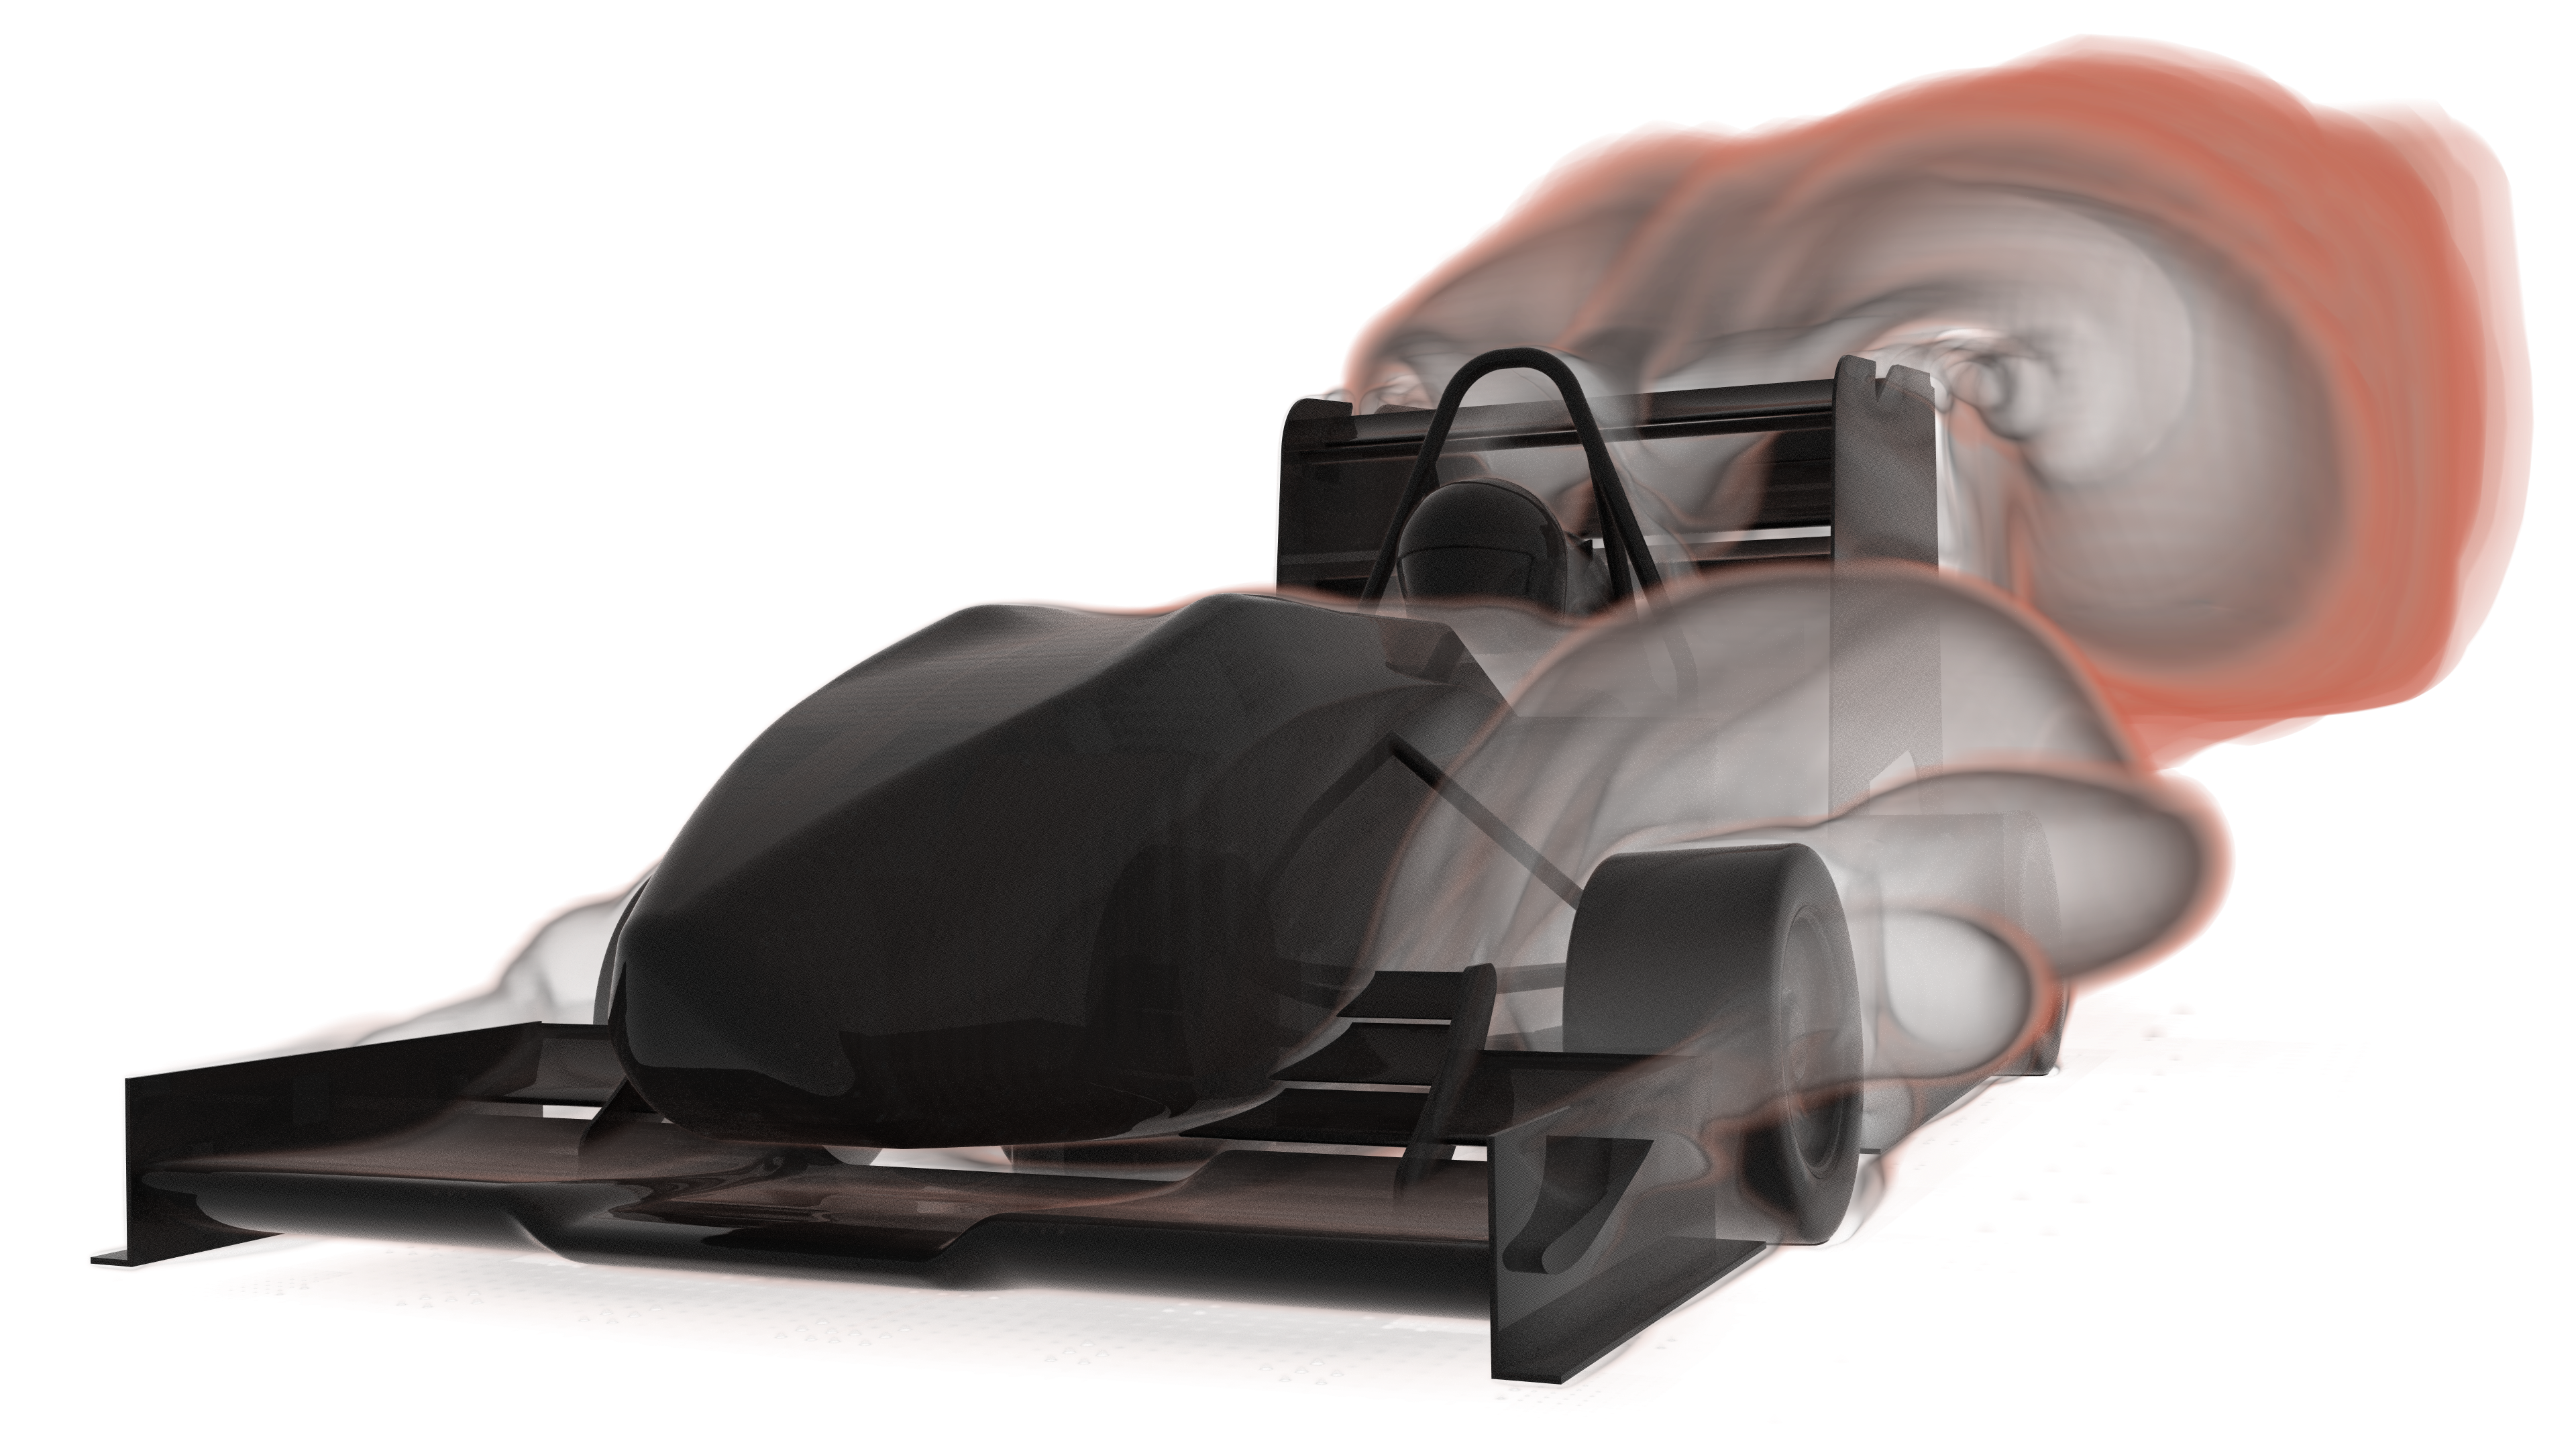
\includegraphics[width=0.9\linewidth]{pics/Titelbild.png}
        \end{figure}
        \vfill
        \normalsize
        % Tabelle angepasst: Nur noch 3 Spalten (Label, Student 1, Student 2)
        \begin{tabular}{rrr}
            \rule{0mm}{1ex}Verfasst von:   & \studentNameone & \studentNametwo \\
            \rule{0mm}{1ex}Matrikelnummer: & \hspace*{+0.5em}\studentMatnrone & \hspace*{+0.5em}\studentMatnrtwo \\
            \rule{0mm}{1ex}Studiengang:    & \studentStudiengangone & \studentStudiengangtwo \\
            \\[2em]
            \rule{0mm}{1ex}Betreuer:       & #5 & \\
            \\[1em]
            \rule{0mm}{1ex}Abgabedatum:    & #6 & \\
        \end{tabular}
    \end{center}
    \pagebreak
}